\documentclass[12pt]{article}
\usepackage[margin=1in]{geometry}
\usepackage{graphicx}
\usepackage{booktabs}
\usepackage{amsmath}

\title{The Effect of Paid Search Advertising on Revenue: \\
A Replication of the eBay Natural Experiment}

\author{Lauren Taylor}

\date{\today}

\begin{document}

\maketitle

\section{Introduction}

The goal of this paper is to estimate the causal effect of paid search advertising on eBay's revenue. Firms spend billions of dollars on search engine marketing (SEM), but measuring its true impact is difficult because users who click on ads may have already intended to visit the site. Blake, Nosko, and Tadelis (2014) address this problem using a large-scale natural experiment in which eBay temporarily turned off paid search advertising in selected markets. This paper replicates the core analysis of that experiment using a difference-in-differences (DID) framework to compare revenue trends between treatment and control markets.

\section{Experimental Setting}

Blake et al. (2014) conducted a field experiment in which eBay stopped bidding on Google AdWords in a subset of geographic markets. Specifically, 65 of the 210 designated market areas (DMAs) were selected for treatment starting on May 22, 2012. In these treatment markets, paid search advertising was turned off for eight weeks, while the remaining DMAs continued their normal advertising activity and served as the control group.

The experiment was not fully randomized. The largest DMAs were excluded from the treatment group, which means the treatment and control markets differ in their baseline revenue levels. Because of this difference, a simple comparison of average revenue between the two groups would not provide a reliable estimate of the advertising effect. Instead, the analysis uses a difference-in-differences approach that compares how revenue changes over time between the treatment and control groups.

\section{Data and Figures}

The dataset contains daily revenue observations for 210 DMAs from April through July of 2012. For each market and date, the data include variables indicating the DMA identifier, whether the market belongs to the treatment or control group, the treatment period, and total revenue. These data allow us to compare revenue patterns before and after the intervention across both groups.

\begin{figure}[h]
\centering
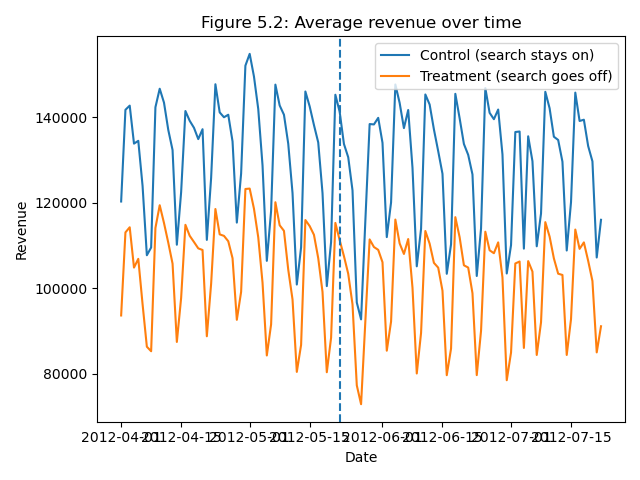
\includegraphics[width=0.85\textwidth]{../output/figures/figure_5_2.png}
\caption{Average revenue for treatment and control DMAs over time.
The dashed line marks May 22, 2012, when SEM was turned off
for the treatment group.}
\label{fig:revenue}
\end{figure}

Figure \ref{fig:revenue} shows the average daily revenue for treatment and control DMAs over time. The control group consistently has higher revenue levels because the largest DMAs were excluded from the treatment group. Both groups also display similar weekly oscillation patterns, which likely reflect regular demand cycles over the week. At this scale, it is difficult to visually detect a clear divergence between the groups after the treatment begins.

\begin{figure}[h]
\centering
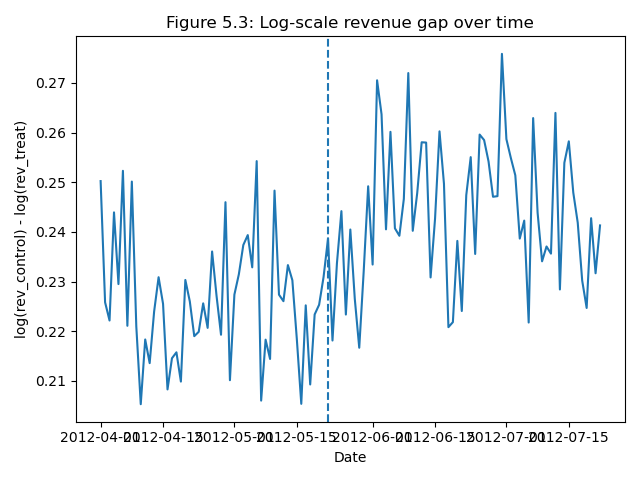
\includegraphics[width=0.85\textwidth]{../output/figures/figure_5_3.png}
\caption{Log-scale average revenue difference between control and treatment
groups over time. The gap appears to increase after May 22.}
\label{fig:logdiff}
\end{figure}

Figure \ref{fig:logdiff} displays the log difference in average revenue between the control and treatment groups. Before May 22, the difference fluctuates around a relatively stable level, suggesting that the two groups follow similar trends prior to the intervention. After the treatment begins, the gap appears to increase slightly, indicating that treatment markets may have experienced a small reduction in revenue relative to the control markets. This visual pattern motivates the use of a formal difference-in-differences estimation.

\section{Results}

\input{../output/tables/did_table.tex}

The difference-in-differences estimate of the treatment effect is $\hat{\gamma} = -0.0066$ in log terms. Converting this estimate into levels implies that treatment markets experienced approximately a 0.66\% decline in revenue after paid search advertising was turned off, since $e^{-0.0066} \approx 0.9934$.

However, the 95\% confidence interval for the estimate is [-0.0175, 0.0043], which includes zero. This means the estimated effect is not statistically significant at the 5\% level. Economically, the results suggest that turning off paid search advertising had only a very small impact on revenue. For a well-known brand like eBay, many users likely reach the website through organic search results rather than through paid advertisements.

\section{Conclusion}

This replication uses a difference-in-differences framework to estimate the effect of paid search advertising on eBay's revenue. The results indicate a small negative effect of approximately 0.66\%, but the estimate is not statistically significant. This finding replicates the main conclusion of Blake et al. (2014), suggesting that paid search advertising has a limited impact on revenue for well-known brands.

There are several limitations to this analysis. The dataset used here contains scaled revenue values rather than the original figures, and the treatment was not fully randomized across markets. Additionally, the analysis relies on a simple DID specification rather than a regression model with additional controls. Despite these limitations, the results provide useful insight into the effectiveness of paid search advertising and highlight the importance of causal identification when evaluating marketing strategies.

\begin{thebibliography}{9}

\bibitem{blake2014}
Blake, T., C. Nosko, and S. Tadelis (2014).
``Consumer Heterogeneity and Paid Search Effectiveness: A Large-Scale Field Experiment.''
\textit{Econometrica}, 83(1): 155--174.

\bibitem{taddy2019}
Taddy, M. (2019).
\textit{Business Data Science}. McGraw-Hill, Chapter 5.

\end{thebibliography}

\end{document}
